%\documentclass[12pt, a4paper]{article}
\documentclass[english,11pt]{report}
\usepackage[utf8]{inputenc}
\usepackage[T1]{fontenc}
\usepackage{natbib}
\usepackage[french]{babel}
\usepackage{amsmath}
\usepackage{graphicx}
\usepackage{wasysym}
\usepackage{diagbox}


%\bibpunct{(}{)}{;}{a}{}{,}
%\bibliographystyle{aa}

\begin{document}

\selectlanguage{english}

\tableofcontents

\chapter{The NIKA2 instrument}
	\section{General description}
	
The New Iram Kid Array-2 (NIKA2) is a next generation camera dedicated to millimeter wave astronomy. It was successfully installed at the IRAM telescope (Sierra Nevada - Spain) in October 2015, replacing its prototype : NIKA. NIKA2 instrument is based on Kinetic Inductance Detectors (KIDs) array technology, which is a novel detectors technology based on superconductivity and provides at the same time high sensitivity and ease of multiplexing. Plus, it is a dual band camera, observing at 2.05 mm and 1.15 mm (corresponding to frequencies of 260 GHz and 150 GHz respectively) thanks to the simultaneous readout of respectively a 1000 pixels array and 2x2000 pixels arrays. The two arrays at 1.2 mm permits the measurement of the linear polarization. The other fundamental components of NIKA2 are : \\

\begin{itemize}
\item A dilution cryostat : To cool down the detector arrays at their ideal working temperature of ~100 mK.
\item Readout electronics : A series of electronics boards named NIKEL. It allows us to acquire the astronomical signal by reading all detectors simultaneously using one single coaxial line.
\item Optics chain : It was designed to have a much larger Field of View (FoV), which is 6.5 arcmin in diameter (1.8' for NIKA). (The FoV describes the angular extent of a given sky area imaged by a camera) \\
\end{itemize}

The Tab \ref{NIKA2} shows the main characteristics of NIKA2.

 \begin{table}[h!]
\center
\begin{tabular}{|c|c|c|c}
  \hline
Wavelength (mm) & 2.0 & 1.2 & 1.2 (Q,U)  \\
	\hline
 Frequency (GHz) & 150 & 260 & 260 \\
  \hline
 FWHM (arcsec)  & 16 (goal) & 10 (goal) & 10 (goal) \\
  \hline
 Number of detectors & 1020 & \multicolumn{2}{l|}{2x1140}  \\
 \hline
 FoV  & 6.5' & 6.5' & 6.5' \\
  \hline
\end{tabular} 

\caption{NIKA2 technical characteristics}
 \label{NIKA2}
\end{table}

\section{Kinetic Inductance Detectors : KIDs}
KIDs are RLC superconducting resonators made from a thin metal film that react with an incoming radiation and change their electromagnetic properties. In fact, when photons are absorbed by the film, they break Cooper pairs in the superconducting element and increase the density of quasi-particles (it changes the ratio of paired (Cooper pair) and unpaired (quasi-particles) charge carriers). As a consequence, the kinetic inductance $L_{k}$ is modified and therefore produces a shift of the resonant frequency of the KID (\textbf{mettre ref Doyle et al 2008}). Finally, the absorbed power can be directly related to the change of  the resonant frequency (\textbf{mettre ref Calvo et al 2013}).

	\subsection{Link between the kinetic inductance and optical power}
Because of the kinetic energy transported by Cooper pairs, the impedance of a superconductor stimulated by an electromagnetic field of angular frequency $w$ is defined by $Z_{s} = R_{s} +jwL_{k}$ ($R_{s}$ take account of losses due to residual electrons).  The kinetic inductance $L_{k}$ is proportional to Cooper pair density (\textbf{D'Addabbo 2014}):

\begin{equation}
\delta L_{k} \propto -\delta(n - n_{qp}) \propto \delta n_{qp}
\end{equation}

	\subsection{Detector response}
	\subsection{Frequency multiplexing}
	
\section{Main scientific axes with NIKA2}

\chapter{Introduction}
Context, CMB mode B, space mission, besoin de matrices de plus en plus grandes : sol = KIDs 

\chapter{KIDs simulations and non-linearity}

The objectif of these simulations is, in a first part, to model the response of a KID when it is submitted to an incoming radiation, and to determine the non-linearity coefficient which is systematic to the detector. And in a second part to determine if this non-linearity can prevent us from detecting the CMB polarization within the context of a space mission. First, we will talk about the response of a KID, then about different methods to reconstruct the signal perceived by the detector, finally we will calculate the non-linearity coefficient for the detector and give a parameter space for which this non-linearity is acceptable.

\section{Kinetic Inductance Detectors : KIDs}
\subsection{Generalities}
KIDs are RLC superconducting resonators made from a thin metal film that react with an incoming radiation and change their electromagnetic properties. In fact, when photons are absorbed by the film, they break Cooper pairs in the superconducting element and increase the density of quasi-particles (it changes the ratio of paired (Cooper pair) and unpaired (quasi-particles) charge carriers). As a consequence, the kinetic inductance $L_{k}$ is modified and therefore produces a shift of the resonant frequency of the KID (\textbf{mettre ref Doyle et al 2008}). Finally, the absorbed power can be directly related to the change of  the resonant frequency (\textbf{mettre ref Calvo et al 2013}).

	\subsection{Response of a KID}
In order to model the comportement of a KID when excited by an incoming radiation, we follow the parametrisation proposed by \cite{2008ApPhL..93m4102G}.

\begin{equation}
S_{21} = \frac{2Z_{res}Z_{0}}{Z_{res}[2Z_{0} + j(X_{1}+X_{2})] + (Z_{0} +jX_{1})(Z_{0} +jX_{2})}
\end{equation}

with :

\begin{equation}
Z_{res} = \frac{Z_{0}Q_{e}}{2Q_{i}}[1 + 2jQ_{i}\frac{(f-f_{0})}{f_{0}}]
\end{equation}

Where $X_{1}$, $X_{2}$, $Z_{0}$ are impedances, $Q_{i}$ is the intrinsic quality factor of the resonator and $Q_{e}$ is the external quality factor due to coupling with the measurement electronics. $f_{0} \sim 1$ GHz, is the resonant frequency of the KID, and $\delta f_{0} \sim 1$ kHz is its variation when the detector is excited. f is the frequency of excitation to which the detector is submitted.\\

$S_{21}$ represents the transfer function of the signal measured.
\begin{equation}
S_{21}(f) = I + jQ
\end{equation}
where I = $Re(S_{21})$ (in phase) and Q = $Im(S_{21})$ (quadrature)\\

METTRE IMAGES I, Q, I vs Q
	\section{Reconstruction du décalage de la fréquence de résonance}
	
When the KID is excited by an incoming radiation, its resonance frequency varies. Thanks to this shift $\delta f_{0}$, we can reconstruct the signal transmitted.\\
For the NIKA2 detectors an innovated readout technique has been developped. The idea is to use an excitation based on two different frequencies instead of using an excitation at a fixed tone. To realize that, we rapidly modulate the local oscillator signal between two readout tones, separated by $\delta f_{LO}$, one just above ($f_{+}$ = $f_{0}$ + $\delta f_{LO}/2$) and one just below ($f_{-}$ = $f_{0}$ - $\delta f_{LO}/2$) the detector resonant frequency $f_{0}$. The modulation $\delta f_{LO}$ is performed at about 1 kHz. This technique allows to measure, for each data sample, I, Q and their variation dI, dQ. Here, I(t) and Q(t) are sampled at 22 Hz, they are the mean values of sub-sample i(t) and q(t) on $N_{m}$ = 40 points at 880 Hz (la fonction de transfert est échantillonnée à 880 Hz, ces échantillons sont moyennés afin de calculer I(t) et Q(t) sur 40 points). dI(t) and dQ(t) are the mean values of the difference between the data measured at $f_{-}$ and $f_{+}$. 

\begin{equation}
I = \sum^{N_{m}=40}_{p=1} i_{p}
\end{equation}

\begin{equation}
Q = \sum^{N_{m}=40}_{p=1} q_{p}
\end{equation}

\begin{equation}
dI = \sum^{N_{m}/2=20}_{p=1} i_{2p} - i_{2p-1}
\end{equation}

\begin{equation}
dQ = \sum^{N_{m}/2=20}_{p=1} q_{2p} - q_{2p-1}
\end{equation}

METTRE SCHEMA CERCLE DE RESONANCE\\

With these four quantities we can reconstruct the signal by applying two different method : RfdIdQ and Pf. 

\subsection{Method RfdIdQ}
When the detector is excited, the optical power is changed by an amount $\Delta P_{opt}$, and a variation $\Delta I(t)$, $\Delta Q(t)$ is observed between successive points. 
dI and dQ are used as a calibration factor to associate to the observed $\Delta I(t)$, $\Delta Q(t)$ the corresponding change in the resonance frequency $\Delta f_{0}$, and hence to reconstruct $\Delta P_{opt}$.

Then we can estimate the shift in the resonant frequency between two samples with : 
\begin{equation}
\Delta (\delta f_{0}(t)) = \delta f_{LO} \frac{\Delta I<dI>_{50} + \Delta Q<dQ>_{50} }{<dI>_{50}^{2} + <dQ>_{50}^{2}}
\end{equation}

$< a >_{50}$ means that we did an average 50 points before and after \textit{a}.\\

The shift of the resonant frequency (and so the variation of the optical power) as a function of time is calculated by integrating the difference between each samples.

\begin{equation}
\delta f_{0}(t) = \sum^{t}_{t'=0} (\Delta \delta f_{0}(t'))
\end{equation}
REF CATALANO 2014

\subsection{Polynomial fit : Pf}
REF FXD 2017\\

The idea of this method is to project I, Q, dI, dQ, onto an axis which is as linear as possible with frequency (and so is assumed to be linear with the optical power). To do so, we have to study the quantity given by GRABOVSKIJ: $Z = I + jQ$. We do the hypothesis that $f=f_{0} +\frac{w}{2} tan\frac{\phi}{2}$.\\
When near a resonance, Z is on a circle. The inverse of Z is a circle, we can normalize it in a way to have an infinite radius circle which can be represented as the axis that is supposed to be linear whith the KID frequency. To do this inversion, we proceed in two phase : 

\begin{itemize}
\item First, we transform the initial circle by scaling, translating and rotating it, so that it is identical to the reference circle wich has $\frac{1}{2}$ radius and is centered on ($\frac{1}{2}$,0) in the complex plane. This circle, $Z_{norm}$ is defined by :

\begin{equation}
\begin{split}
Z_{norm} & = \frac{1}{2} + \frac{1}{2}e^{i\varphi} \\
& =  \frac{1}{2} + \frac{1}{2} (cos\varphi + isin\varphi) \\
 & = \frac{1}{2}(1+cos\varphi) + \frac{i}{2} sin\varphi \\
 & = \frac{1}{2} (1+ cos\varphi) +\frac{i}{2} sin\varphi \\
  & = \frac{1}{2} (2cos^{2}\frac{\varphi}{2}) + i sin\frac{\varphi}{2}cos\frac{\varphi}{2} \\
  Z_{norm}  & = cos\frac{\varphi}{2}  e^{i\frac{\varphi}{2}}
\end{split}
\label{Znorm}
\end{equation}

\item Secondly, we inverse the circle : $Z_{res} = \frac{1}{Z_{ref}}$
\begin{equation}
\begin{split}
Z_{res} & = \frac{1}{cos\frac{\varphi}{2}}  e^{-i\frac{\varphi}{2}}\\
 & = \frac{1}{cos\frac{\varphi}{2}}(cos(-\frac{\varphi}{2}) + isin(-\frac{\varphi}{2})\\
 Z_{res}& = 1 - i tan\frac{\varphi}{2}
\end{split}
\label{Zres}
\end{equation}
\end{itemize}

We note that the imaginary part of $Z_{res}$ is linearly dependant on the frequency (hyp). So the axis (we will call it $y_{3}$) on which we "project" I, Q, dI and dQ corresponds to $Im(Z_{res})$. To calibrate this dependency we use the dI and dQ measurements which we obtain from the modulation. \\

To compute the first phase, we do a fit of the circle (I vs Q) to find its properties : the radius r, its center ($x_{c}$,$y_{c}$) and its rotation angle $\alpha = atan \frac{yc}{xc}$. After applying the transformation, Z becomes $Z_{norm}$ with :

\begin{equation}
I_{norm} = - \frac{1}{2r}[(I-x_{c})cos\alpha + (Q - y_{c})sin \alpha] + \frac{1}{2}
\end{equation}
\begin{equation}
 Q_{norm} = \frac{1}{2r}[-(I-x_{c})sin\alpha + (Q - y_{c})cos \alpha] 
\end{equation}

To calibrate $y_{3}$, which is assumed to be proportional to $f-f_{0}$, we use dI and dQ, the measured variations of the signal with a modulation of frequency  $\Delta f$. We obtain : 
\begin{equation}
dI_{norm} = -\frac{1}{2r}(dI cos\alpha + dQ sin\alpha)
\end{equation}

\begin{equation}
dQ_{norm} = \frac{1}{2r}(-dI sin\alpha + dQ cos\alpha)
\end{equation}

The derivative of the inverse complex is $dZ_{res} = -\frac{dZ_{norm}}{Z_{norm}^{2}}$. To calibrate $y_{3}$ we use $dy_{3}$ which is the imaginary part of $dZ_{res}$. To do so, we fit $ \frac{\Delta f }{dy_{3}} = R_{n}(y_{3})$ where $R_{n}$ is a polynomial function of degree n. Then, we can easily integrate  $R_{n}(y_{3})$ into $P_{n+1}(y_{3})$ and obtain the relative frequency of the KID with $f-f_{0} = P_{n+1}(y_{3})$.\\

(comparer les 2 methodes )

 \section{KIDs non-linearity}
 \subsection{Comparison of Rf and Pf}
 
 \begin{figure}[h]
\center
	\includegraphics[scale=0.5]{NL_rf.eps}
	\caption{Evolution of KIDs non-linearity as a function of an incoming flux}
	\label{star}
\end{figure}
 \subsection{Non-linearity coefficients and space parameter}

The non-linearity is defined by : $m = m_{1} + \varepsilon m_{1}^{2}$, with $m$ a measure done by the KID. We calculate the non-linearity coefficient $\varepsilon$ of the detector by fitting the incoming flux as a function of the outcoming flux with a polynom of degree 2. Table \ref{Results} give the non-linearity coefficients found by using the Rf and Pf methods, anb by varying the incoming flux.

 \begin{table}[h!]

\center
\begin{tabular}{|c|c|c|}
  \hline
 \backslashbox{$f_{in}$ (Hz)}{$\varepsilon$} & $\varepsilon_{R_{f}}$ & $\varepsilon_{P_{f}} $ (a mettre a jour) \\
	\hline
 $10^{1}$  & - 2,24 x $10^{-6}$ & - 3,60 x $10^{-8}$ \\
  \hline
 $10^{2}$ & - 5,87 x $10^{-7}$ & 1,21 x $10^{-9}$ \\
  \hline
 $10^{3}$  & - 7,71 x $10^{-7}$ & 4,18 x $10^{-12}$ \\
  \hline                                         
 $10^{4}$  & - 2,62 x $10^{-6}$ & 6,25 x $10^{-8}$ \\
  \hline
\end{tabular} 

\caption{Non-linearity coefficients for Rf and Pf methods}
 \label{Results}
\end{table}




In order to construct a space parameter for which the non-linearity induced by a KID is acceptable (here meaning that the detection of B-mode polarization of the CMB is not contaminated by the KID systematics effects), we compare $\varepsilon$ with a non-linearity coefficient, $\varepsilon'$, attached to the measurement, $m$, of the CMB.\\

We have : $m_{1} = T + P$  \\ 
We add the non-linearity : $ m = m_{1} + \varepsilon' m_{1}^{2}$

\begin{equation}
\begin{split}
m & = m_{1} +\varepsilon' (T+P)^{2} \\
& = m_{1} + \varepsilon'(T+P)^{2}  \\
 & =  m_{1} + \varepsilon'(T^{2} + P^{2} + 2TP) \\
 & = T + P + \varepsilon'(T^{2} + P^{2} + 2TP) 
\end{split}
\end{equation}

with $\varepsilon' \ll 1$ et $T = I, P = Q\cos(2\alpha) + U \sin(2\alpha)$

\begin{equation}
\begin{split}
m & =  I + Q\cos(2\alpha) + U\sin(2\alpha) + \varepsilon' [I^{2} +(Q\cos(2\alpha) + U\sin(2\alpha))^{2} + 2I(Q\cos(2\alpha) + U\sin(2\alpha))]\\
& = I  + Q \cos(2\alpha) + U \sin(2\alpha) + \varepsilon' [I^{2}  + (Q\cos(2\alpha))^{2} + (U \sin(2\alpha))^{2} + 2QU\cos(2\alpha)\sin(2\alpha) \\
& + 2IQ\cos(2\alpha) + 2IU\sin(2\alpha)] \\
& \simeq (I + \varepsilon' I^{2}) + (Q + 2\varepsilon' IQ) \cos(2\alpha) + (U + 2 \varepsilon' IU) \sin(2\alpha)
\end{split}
\label{eq-NL}
\end{equation}

To calculate $\varepsilon'$, we generate I, Q, U maps from observed $C_{l}$, to wich we apply the non-linear mapping described by the equation \ref{eq-NL}. This will generate spurious components such as BB signal. METTRE CARTES.
We find : $\varepsilon'$ = 4,44 x $10^{-7}$.
Espace de parametres ?\\
CCL

\chapter{Simulation of sky observations}


\section{Strategie d'observation}
Simulation of "une strategie d'observation typique" (ex : Planck)
Montrer que on est dans le bon espace de parametres.

\section{}
$C_{l}$ calculation\\
Application du mapping NL, sortie du coeff de NL


\section{Addition of dipoles and foregrounds }


%On compare alors le coefficient de NL trouvé avec HEALPIX $\varepsilon'$ avec celui trouvé avec les simu KIDs $\varepsilon$. Pour pouvoir avoir une chance de détecter CMB il faudrait que  $\varepsilon$ soit inférieur à $\varepsilon'$ ainsi on éviterait d'etre contaminé par des effets systématiques. \\


%\textbf{Résultats} \\
%
%Rq : Des flux avec amplitudes à 1000 Hz (1 kHz, correspond aux planètes) correspondent à des flux beaucoup pus forts que le CMB, et par conséquent ne devraient pas nous géner pour les simulations.

%Avec les calculs sur les spectres du CMB (cl.pro) on trouve $\varepsilon' \simeq 3,81$x$10^{-7}$.
%On remarque que le coefficient de NL pour les flux faibles n'est que dix fois inférieur à celui pour les flux forts...

%Est ce qu'on ne pourrait pas alors, écrire un petit module qui prend des
%Cl théoriques, génère des cartes I,Q et U, en déduit les cartes I +
%\gamma I^2, Q + 2\gamma IQ et U+2\gamma IU, faire passer Anafast pour
%avoir des Cl modifiés, qu'on pourrait alors passer à Quickpol ? On fait
%notre Monté-Carlo là-dessus...
%
%la 1ere étape est en effet de générer une carte IQU avec synfast, y appliquer le mapping non-linéaire que tu décris, en prendre le C(l) avec anafast,
%et regarder ce C(l) dans les yeux (ie différence avec le C(l) d’entrée), afin de se construire une intuition sur la sensibilité de BB a gamma par exemple.


\bibliographystyle{unsrt}

\bibliography{biblio}


\end{document}